\section{Durchführung}
\label{sec:Durchführung}

\subsection{Elektronenstrahl im E-Feld}
\begin{figure}[H]
  \centering
  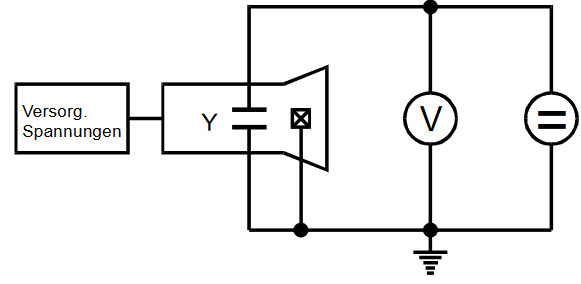
\includegraphics[height=6cm]{Elektronenstrahlroehre_Schaltung.PNG}
  \caption{Schaltung einer Kathodenstrahlröhre. \cite{sample}}
  \label{fig:Schaltung}
\end{figure}

Die Elektronenkanone der Elektronenstahlröhre wird entsprechen Abbildung \ref{fig:kathode}
an eine Heizspannug $U_G$ sowie die weiteren Fokussierungs- und Beschleunigungsspannungen angeschlossen.
Anschließend werden auch die Ablenkplatten der Röhre, wie in Abbildung \ref{fig:Schaltung} zu erkennen, mit Spannung
versorgt und geerdet. 

Die Fokussierungsspannungen werden nun so eingestellt, dass ein möglichst kleiner leuchtender Punkt auf dem
Detektorschirm zu sehen ist. Bei konstanter Beschleunigungsspannung wird dann die Ablenkspannung variiert, sodass
der Punkt auf der untersten der 9 äquidistantne Linien des Schirms liegt. Die Ablenkspannung dieser Konfiguration wird
notiert. Anschließend wird der Punkt auf die nächst höhere Linie gelegt und die Spannung erneut gemessen.
Dieser Vorgang wird für alle der 9 besagten Linien und für ingesamt 5 unterschiedliche Beschleunigungsspannungen wiederholt.

\begin{figure}[H]
  \centering
  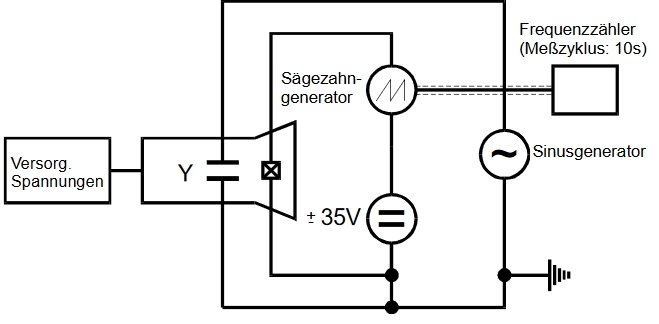
\includegraphics[height=6cm]{Oszilloskop_Schaltung.PNG}
  \caption{Prinzipielle Schaltung eines Kathodenstrahl-Oszillographen . \cite{sample}}
  \label{fig:Schaltung1}
\end{figure}

Im zweiten Teil des Versuchs werden die Ablenkplatten dann an eine Sägezahnspannung (X-Richtung)
und eine Sinusspannung (Y-Richtung) angeschlossen (Abbildung \ref{fig:Schaltung1}). Durch Variation
der Frequenz der Sägezahnspannung wird dann versucht die gewünschten Frequenzverhältnisse
der Spannungen herzustellen. Erkannt werden diese an den stehenden Bildern auf dem
Detektorschirm sowie der dann auf ihm abzählbaren Anzahl an dargestellten Halbwellen.
Die entsprechenden Frequenzen der Sägezahnspannung sowie die maximalen Strahlauslenkungen der Sinusspannung
dieser Konfigurationen werden mithilfe eines Frequenzzählers bzw. der Markierungen des Detektorschirms
gemessen und notiert.
